\documentclass[dissertation.tex]{subfiles}
\begin{document}

\chapter{Exploration of learned representations}

\section{Token-level embeddings}

Filter to notes

\begin{figure}[htpb]
    \centering
    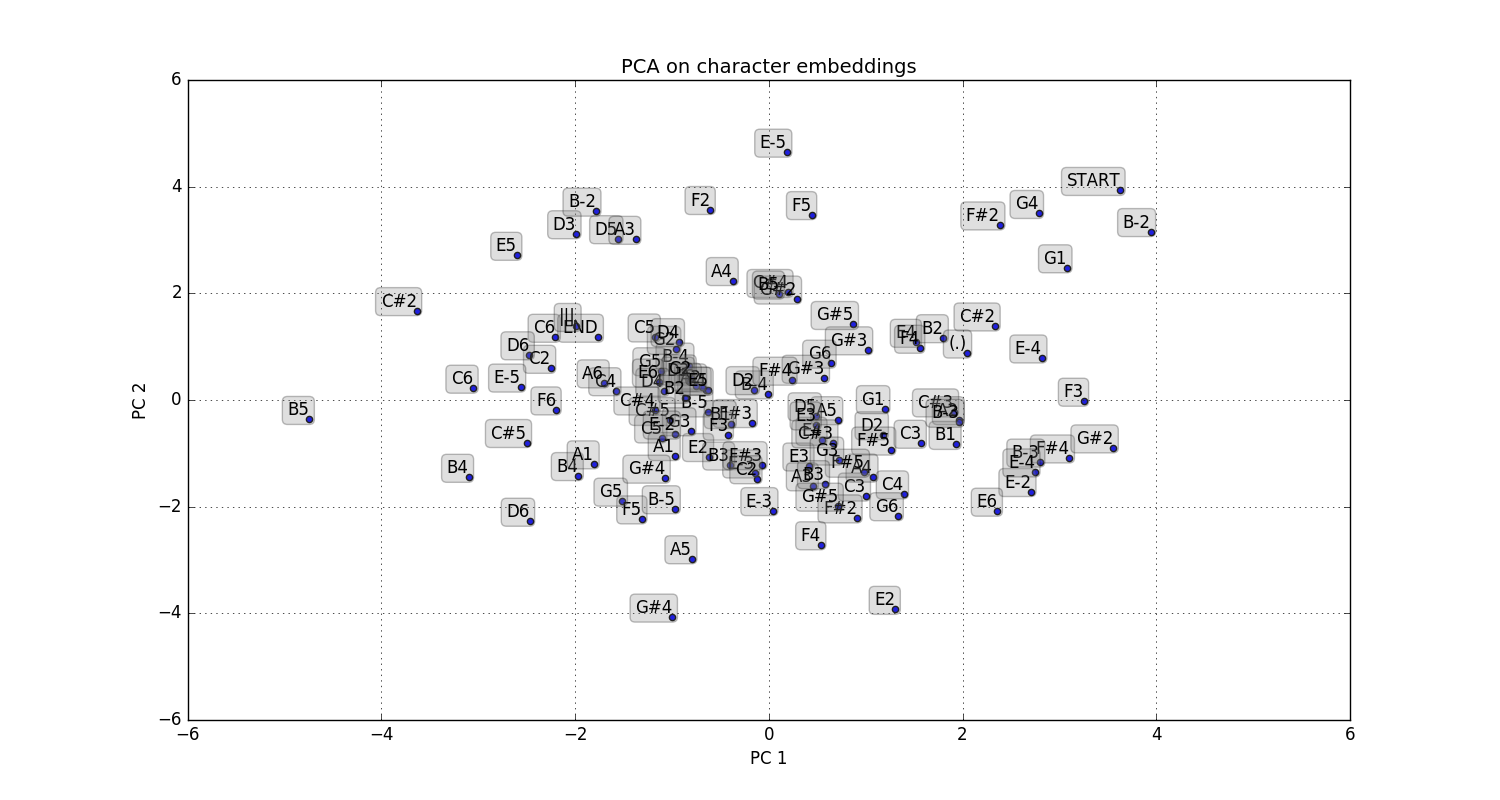
\includegraphics[width=1.0\linewidth]{Figures/PCA-notes.png}
    \caption{PCA embedding of note tokens}
    \label{fig:pca-notes}
\end{figure}

\begin{figure}[htpb]
    \centering
    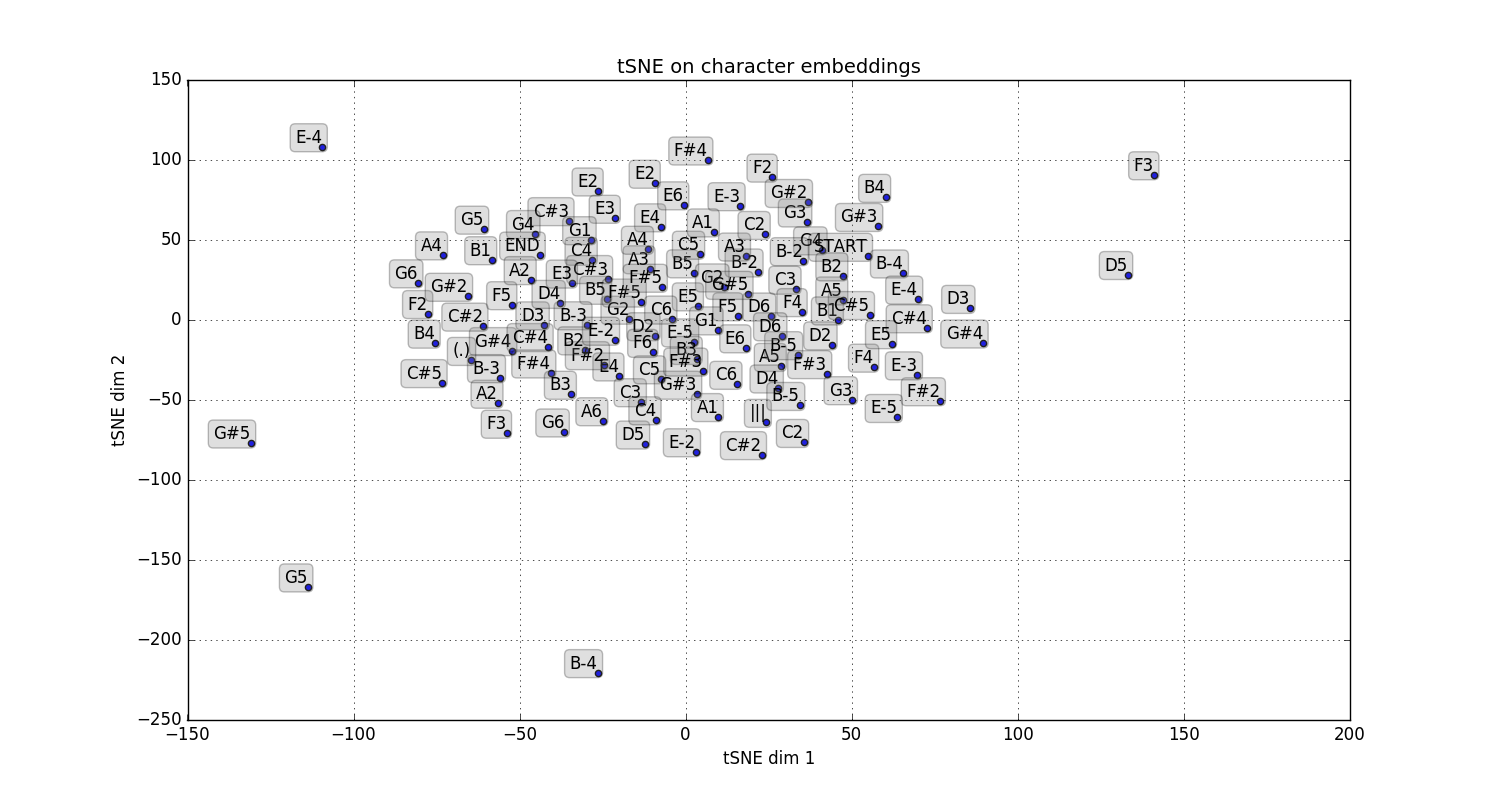
\includegraphics[width=1.0\linewidth]{Figures/tSNE-notes.png}
    \caption{tSNE embedding of note tokens}
    \label{fig:tsne-notes}
\end{figure}

\subsection{Variable-length embeddings}

\todo{LSTM hidden state after consuming chord (chord boundary, do they
    cluster?), phrase (up to fermata, do similar phrases embed similarly),
    whole pieces (difficult to evaluate)}

\section{Memory cells exhibit sensitivity to musical concepts}

One method for gaining insight into what a connectionist model has learned is
to apply some stimulus and measure neuron activations at different layers.

We use as stimulus the music score shown in
\autoref{fig:model-analysis-stimulus}, which has been preprocessed according to
\todo{cite preprocessing}. To aid in relating neuron activities back to music
theory, chords are annotated with Roman numerals obtained using {\tt music21}'s
automated analysis.

\begin{figure}[htpb]
    \centering
    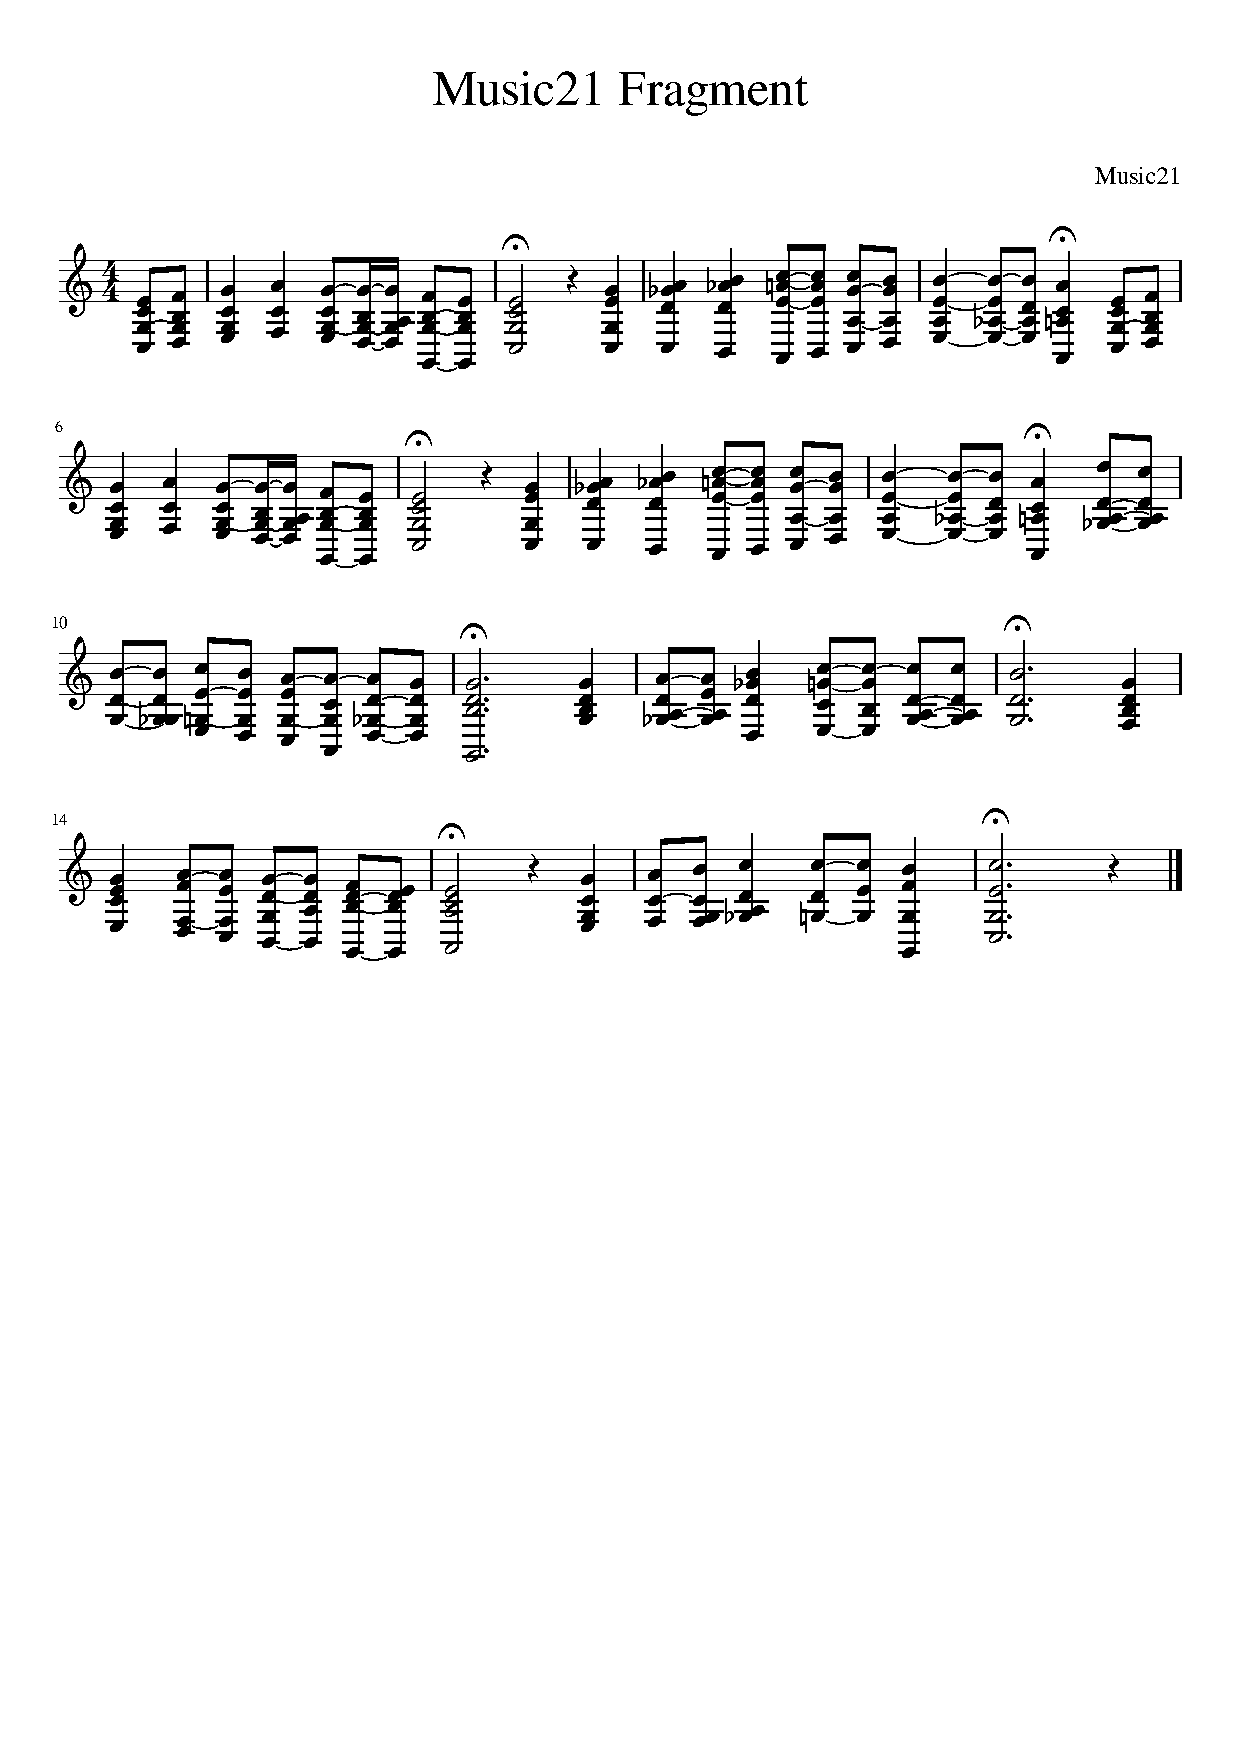
\includegraphics[trim={0 15cm 0 0},clip,width=0.9\linewidth]{Figures/model-analysis-input-score.pdf}
    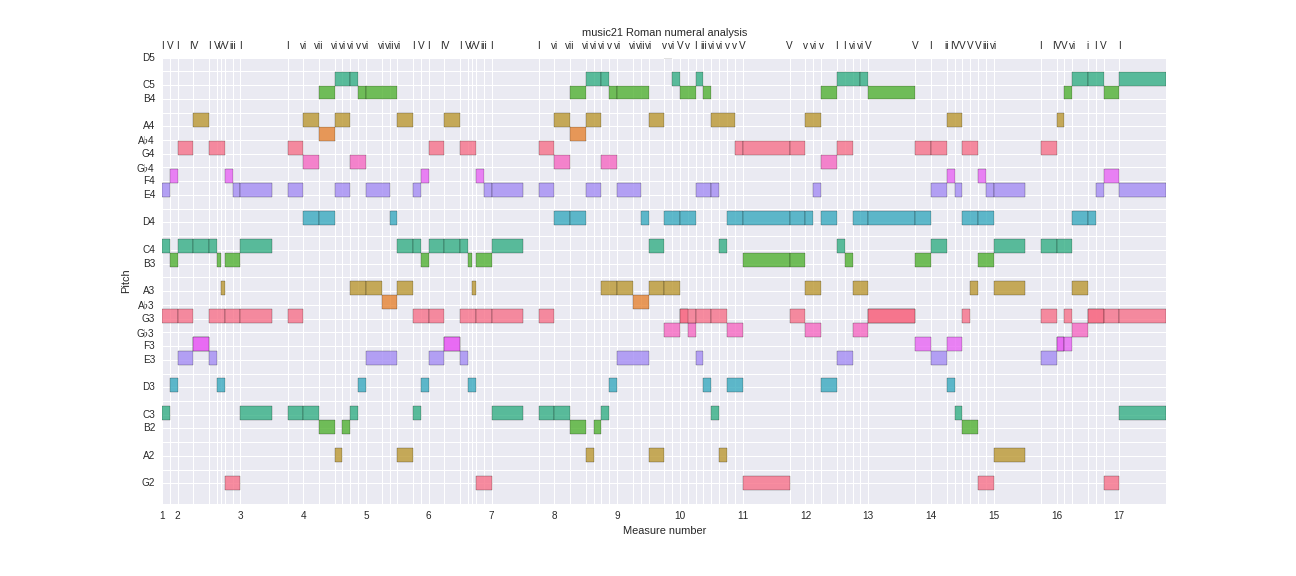
\includegraphics[width=1.00\linewidth]{Figures/model-analysis-input-piano-roll.png}
    \caption{{\it Top}: The preprocessed score (BWV 133.6) used as input stimulus with Roman numeral analysis annotations obtained
        from {\tt music21}; {\it Bottom}: The same stimulus represented on a piano roll}
    \label{fig:model-analysis-stimulus}
\end{figure}

In \autoref{fig:model-analysis-tokens} we visualize the network activations as
the stimulus is sequentially applied. Note that as a consequence of the
variable-length encoding format described in \todo{ref}, the horizontal axis
(number of tokens processed) does correspond directly to time. Rather, time
is advanced one frame every time a chord boundary delimiter symbol is output.

\begin{figure}[htpb]
    \centering
    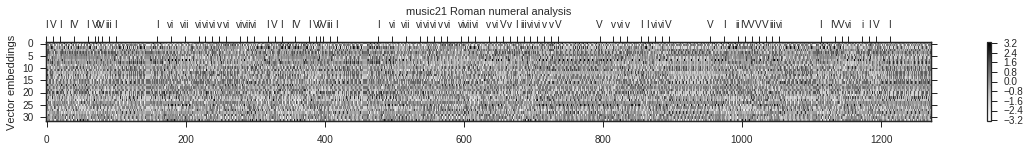
\includegraphics[width=1.0\linewidth]{Figures/model-analysis-tokens-0.png}
    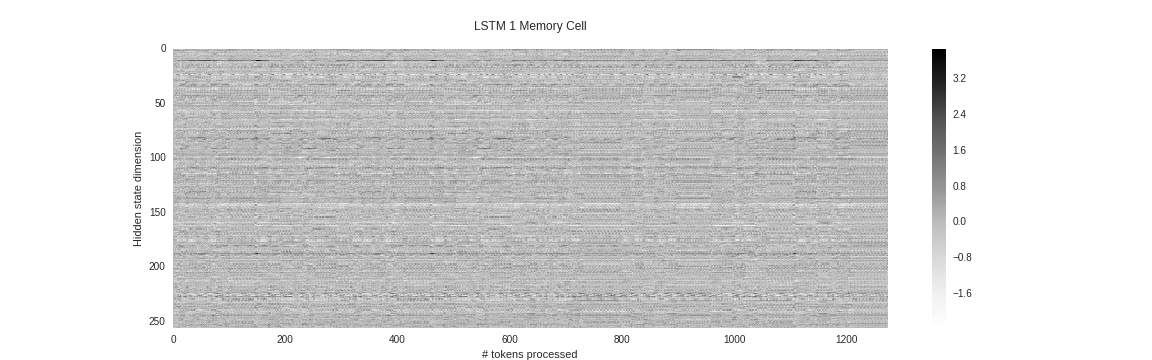
\includegraphics[width=1.0\linewidth]{Figures/model-analysis-tokens-1.png}
    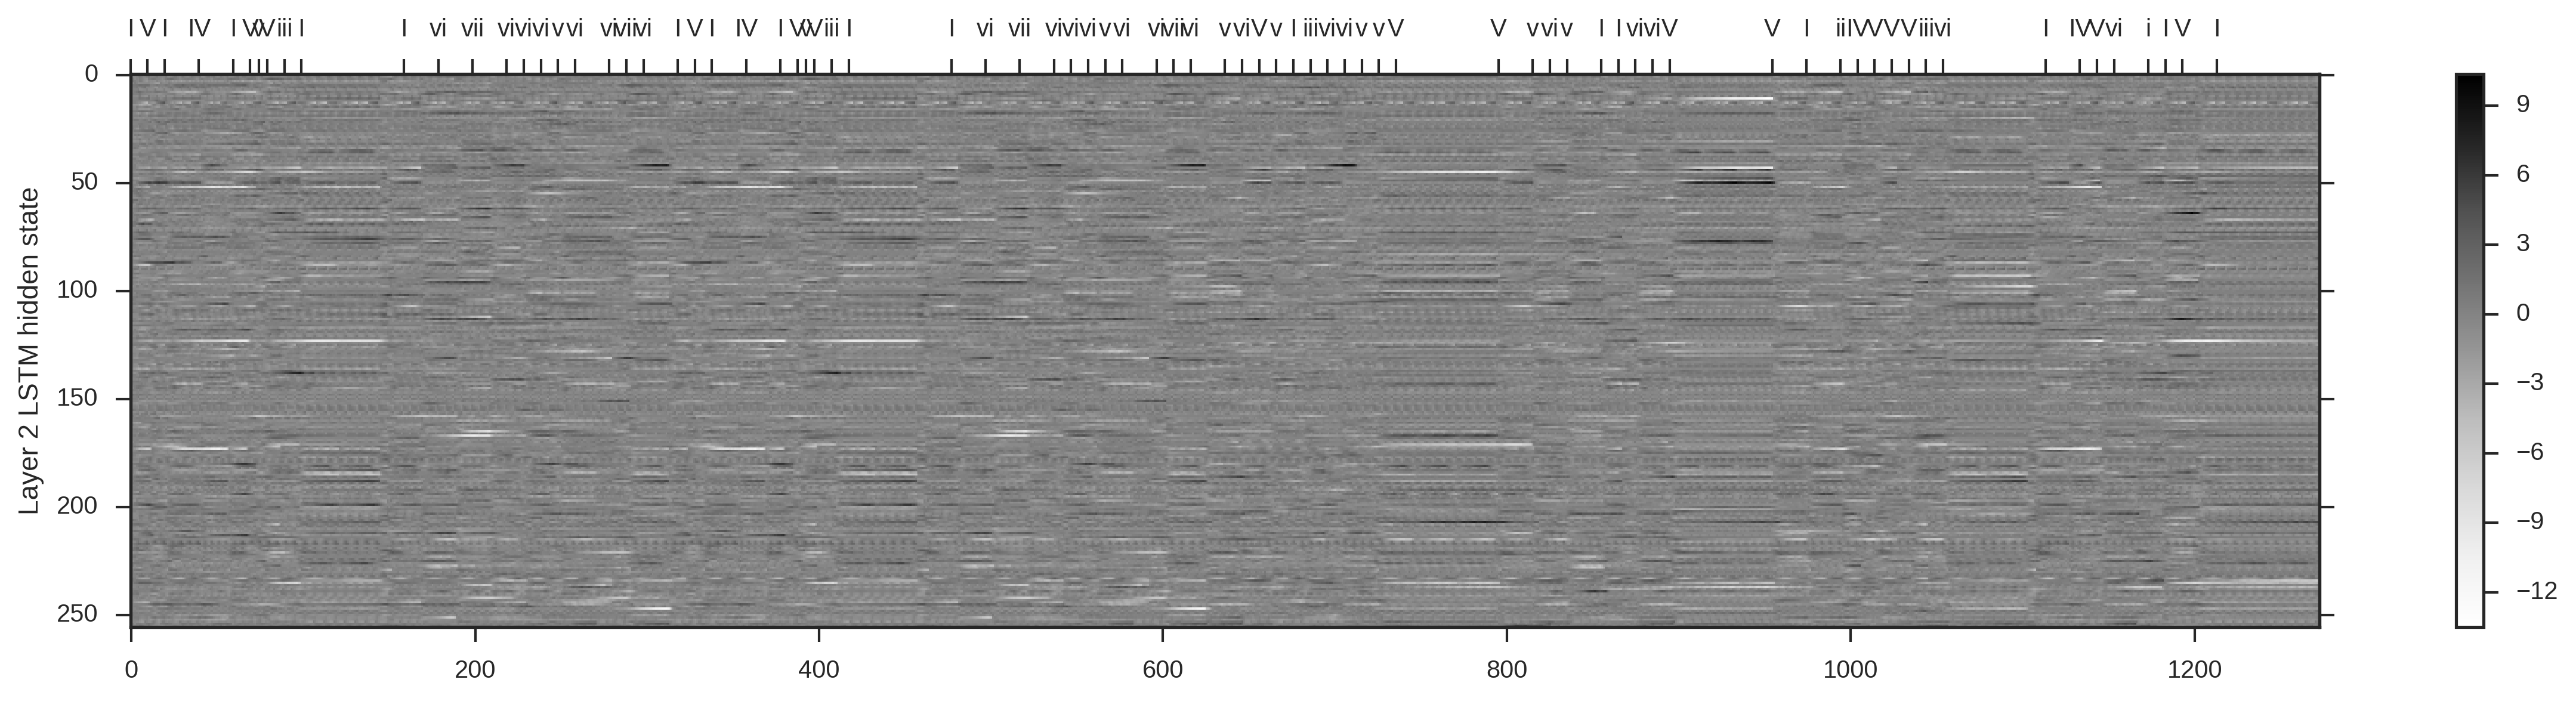
\includegraphics[width=1.0\linewidth]{Figures/model-analysis-tokens-2.png}
    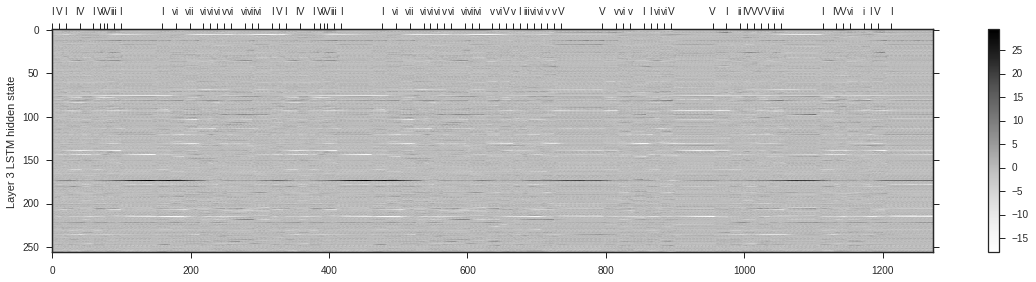
\includegraphics[width=1.0\linewidth]{Figures/model-analysis-tokens-3.png}
    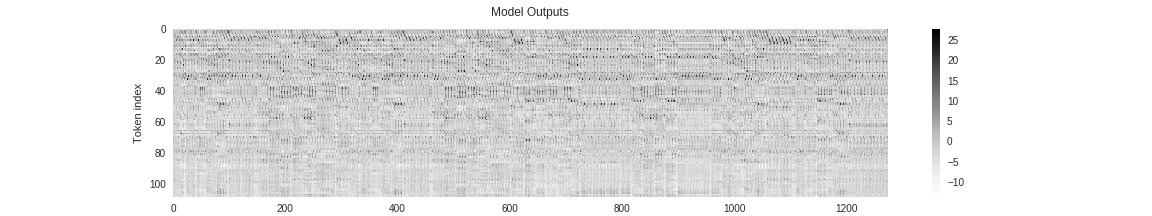
\includegraphics[width=1.0\linewidth]{Figures/model-analysis-tokens-4.png}
    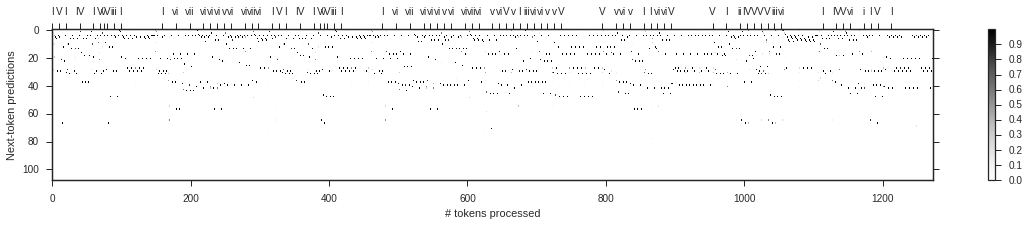
\includegraphics[width=1.0\linewidth]{Figures/model-analysis-tokens-5.png}
    \caption{Neuron activations over time as the encoded stimulus is processed token-by-token}
    \label{fig:model-analysis-tokens}
\end{figure}

\subsection{Pooling over frames}

In order to align and compare the activation profiles with the original score,
all the activations occuring in between two chord boundary delimiters must be
combined. This aggregation of neuron activations from higher resolution (i.e.
note-by-note) to lower resolution (i.e. frame-by-frame) is reminiscent of
pooling operations in convolutional neural networks\todo{cite}. Motivated by
this observation, we introduce the method for pooling an arbitrary number of
token-level activations into a single frame-level activation.

Let $\z^{(l)}_{{t_m}:{t_n}}$ denote the activations of layer $l$ from the $t_m$th input token $\x_{t_m}$
to the $t_n$th input token $\x_{t_n}$. Suppose that $\x_{t_m}$ and $\x_{t_n}$ are respectively the
$m$th and $n$th chord boundary delimiters within the input sequence. Define the
\textbf{max-pooled frame-level activations} $\tilde{\z}^{(l)}_n$ to be the
element-wise maximum of $\z^{(l)}_{{t_m}:{t_n}}$, concretely:
\begin{equation}
    \tilde{\z}^{(l)}_n \coloneqq \left[
        \max_{t_m < t < t_n} \z^{(l)}_{t,1},
        \max_{t_m < t < t_n} \z^{(l)}_{t,2},
        \cdots,
        \max_{t_m < t < t_n} \z^{(l)}_{t,N^{(l)}}
    \right]^\tp
\end{equation}
where $\z^{(l)}_{t,i}$ is the activation of neuron $i$ in layer $l$ at time $t$
and $N^{(l)}$ is the number of neurons in layer $l$. Notice that the pooled
sequence $\tilde{\z}$ is now indexed by frames rather than by tokens and hence
corresponds to time-steps.

We choose to perform max pooling because it preserves the maximum activations
of each neuron over the frame. While pooling methods (e.g. sum pooling, average
pooling) are possible, we did not find significant differences in the
visualizations produced.

\begin{figure}[htpb]
    \centering
    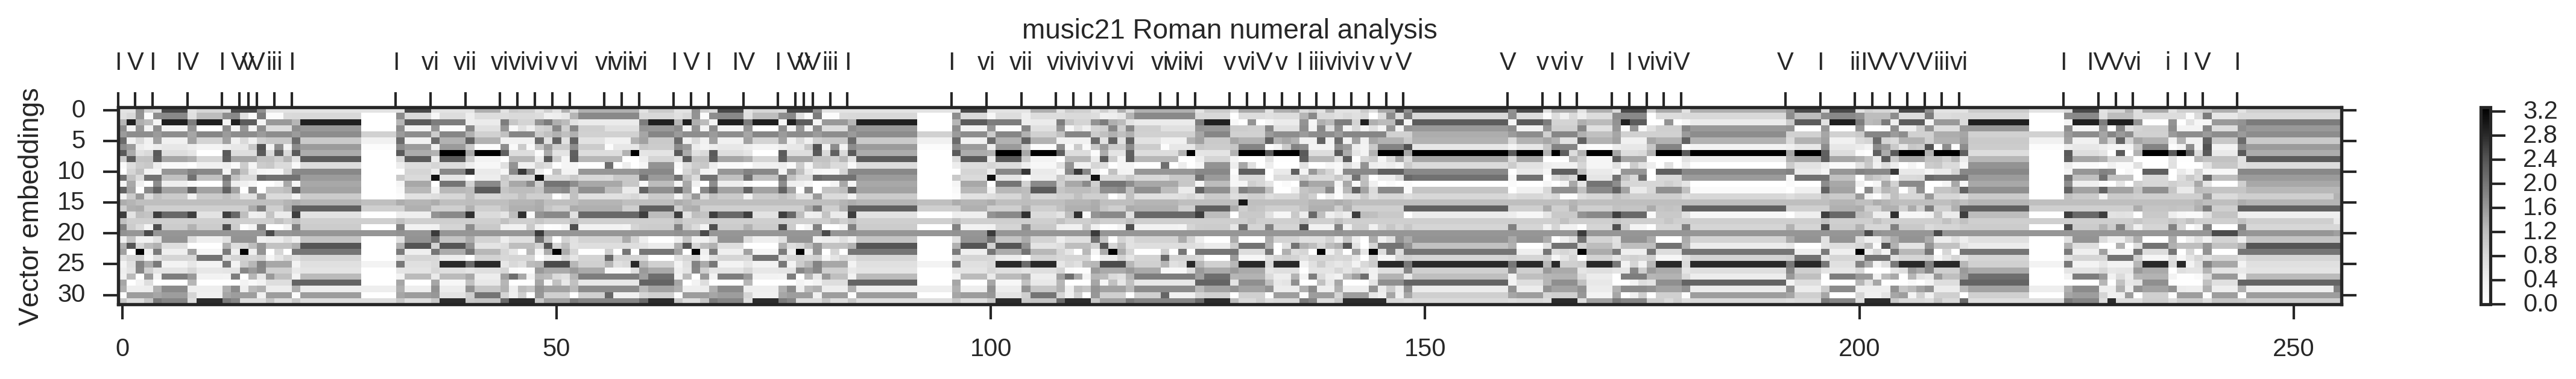
\includegraphics[width=1.0\linewidth]{Figures/model-analysis-chords-0.png}
    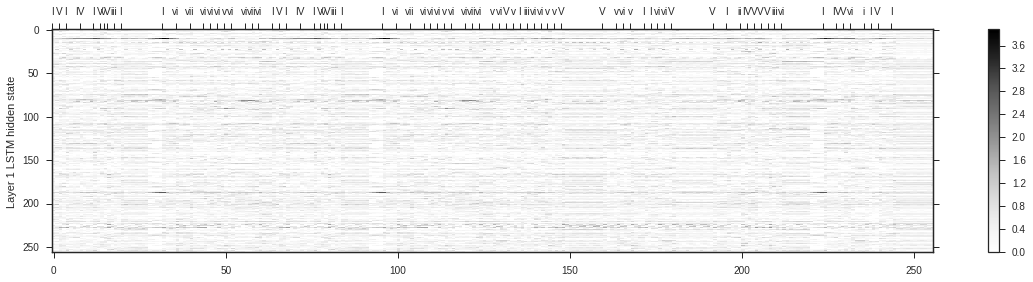
\includegraphics[width=1.0\linewidth]{Figures/model-analysis-chords-1.png}
    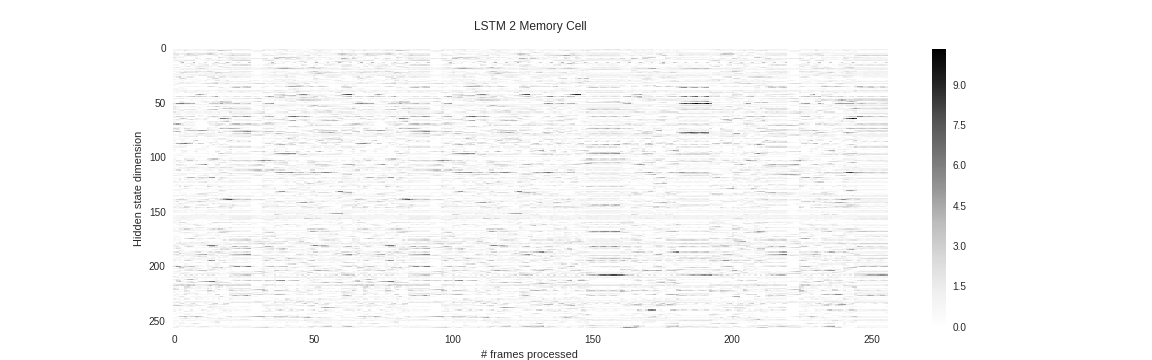
\includegraphics[width=1.0\linewidth]{Figures/model-analysis-chords-2.png}
    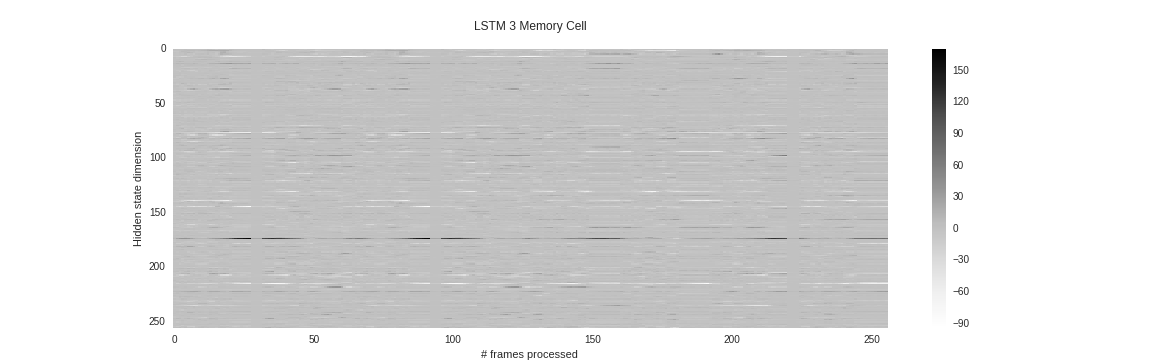
\includegraphics[width=1.0\linewidth]{Figures/model-analysis-chords-3.png}
    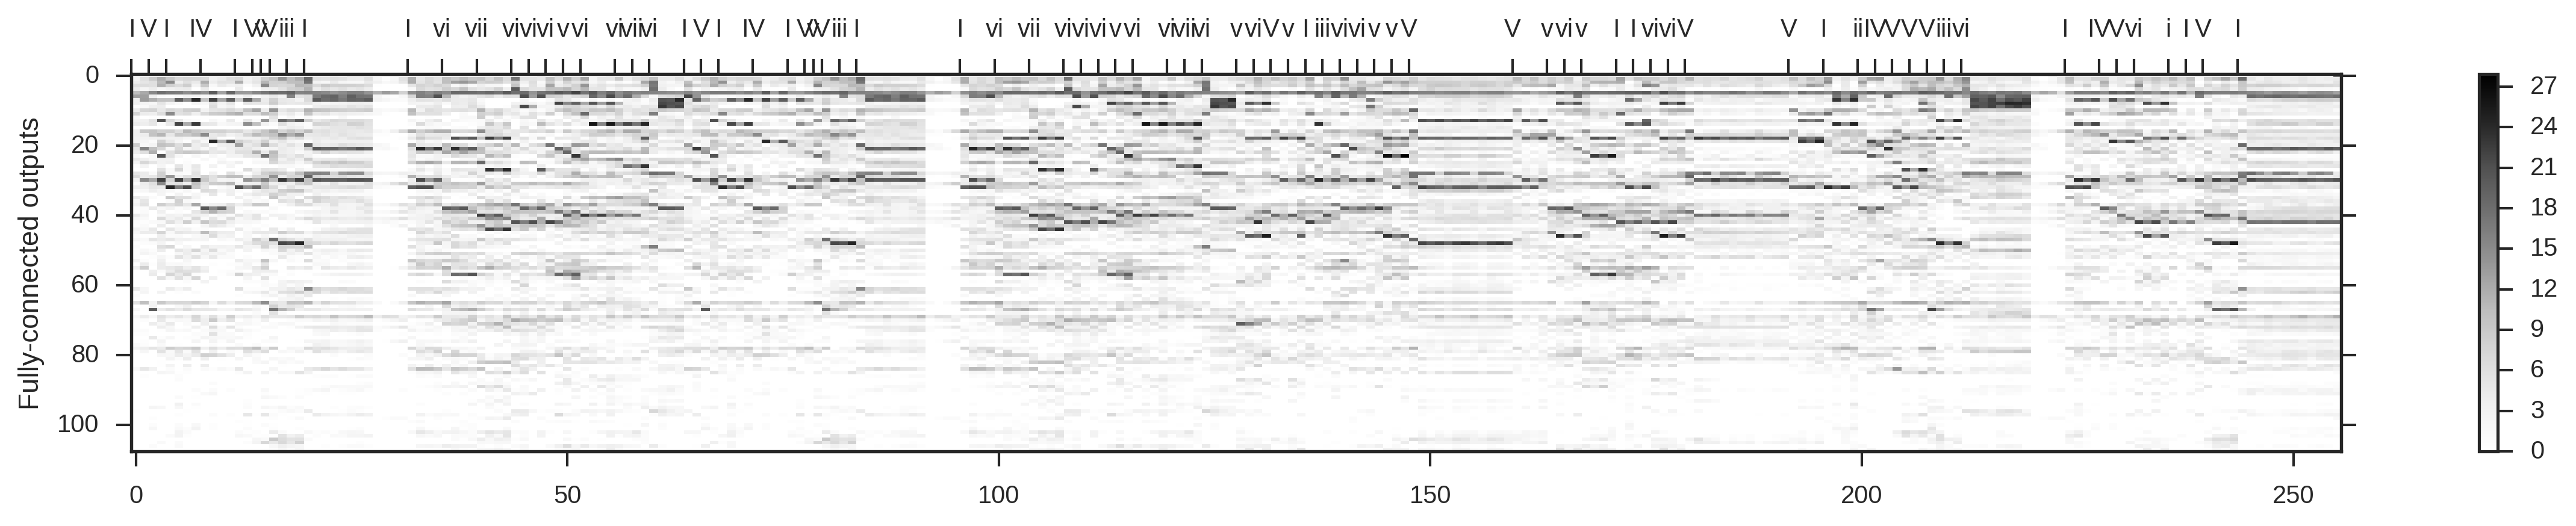
\includegraphics[width=1.0\linewidth]{Figures/model-analysis-chords-4.png}
    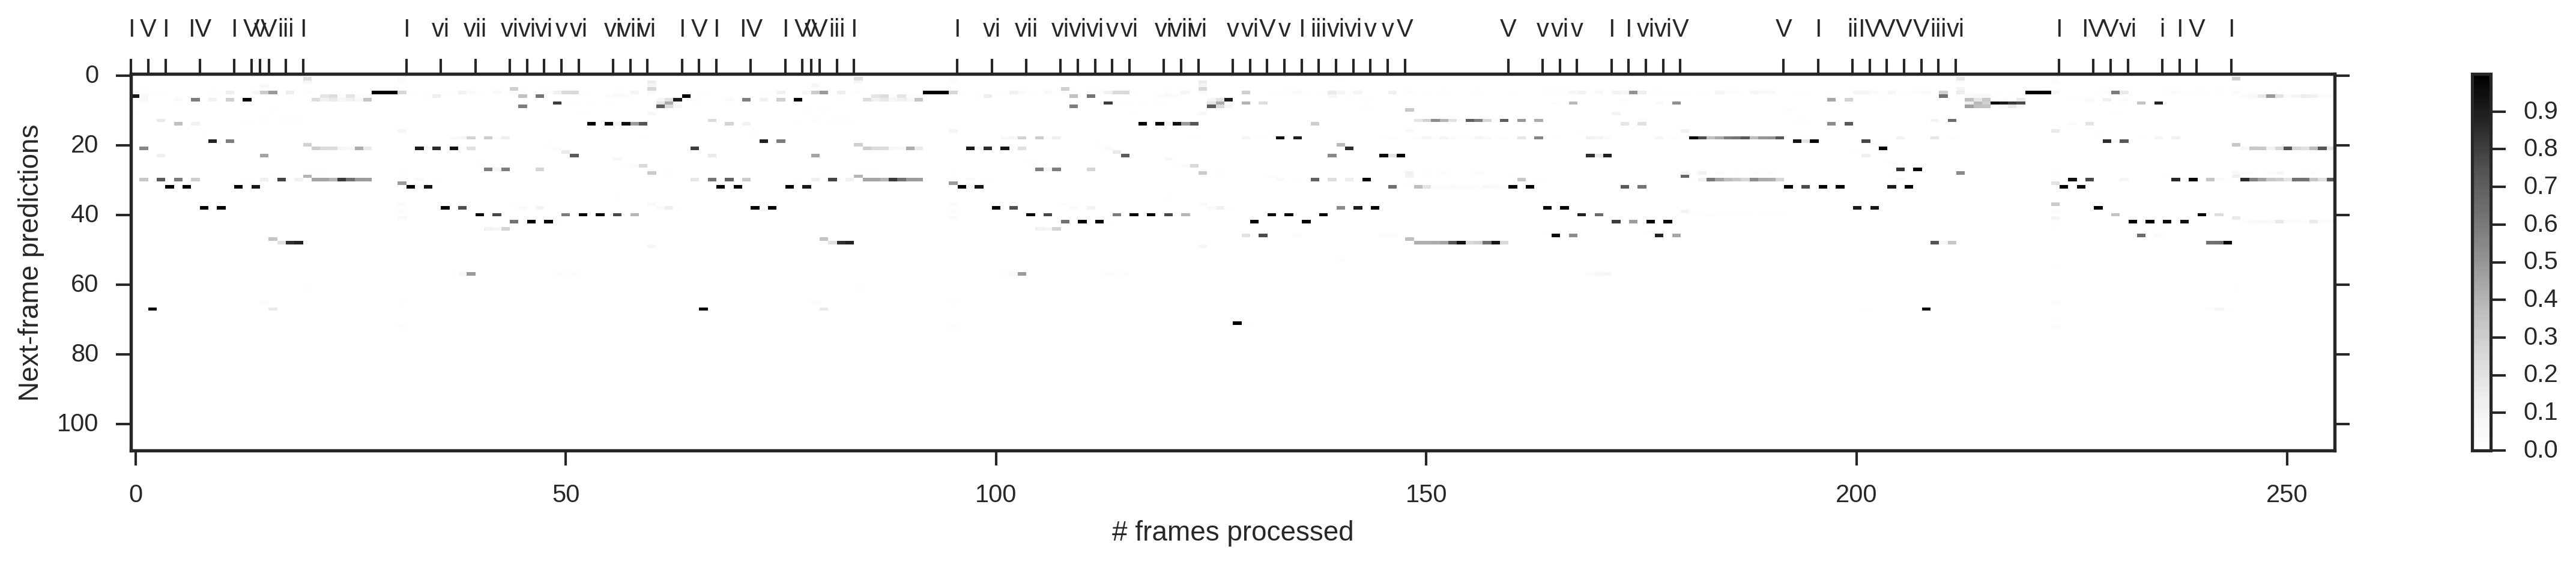
\includegraphics[width=1.0\linewidth]{Figures/model-analysis-chords-5.png}
    \caption{Neuron activations over time pooled over frames}
    \label{fig:model-analysis-frames}
\end{figure}

\begin{equation}
     \coloneqq
\end{equation}

\autoref{fig:model-analysis-probabilistic-piano-roll} shows the next-chord
predictions

probabilistic piano
roll

\begin{figure}[htpb]
    \centering
    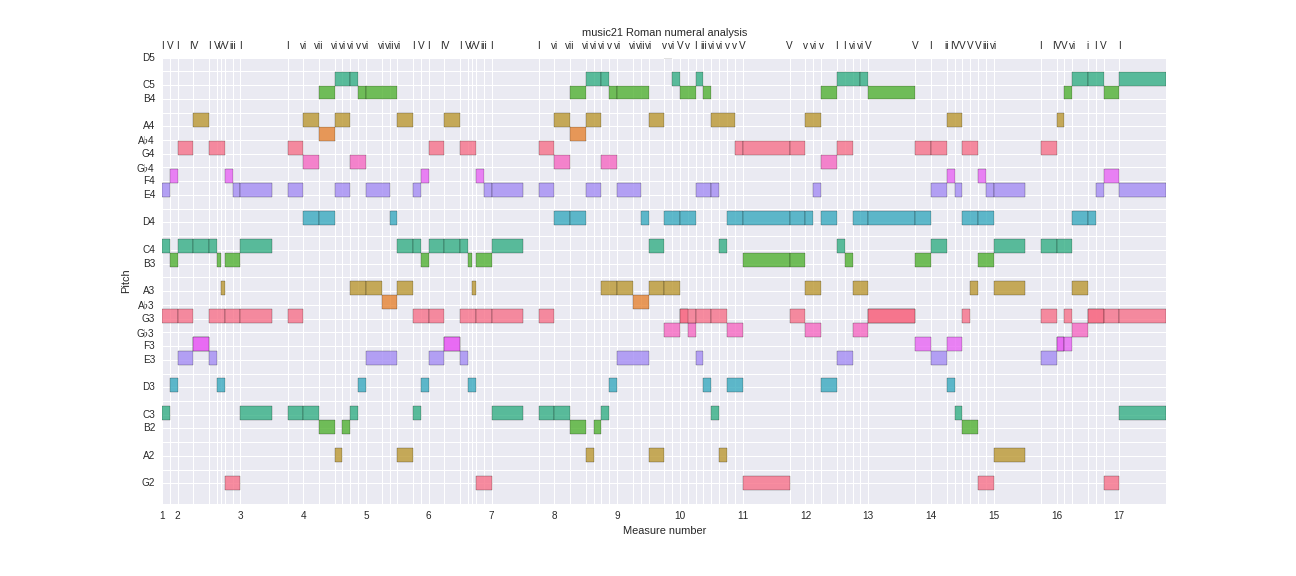
\includegraphics[width=1.0\linewidth]{Figures/model-analysis-input-piano-roll.png}
    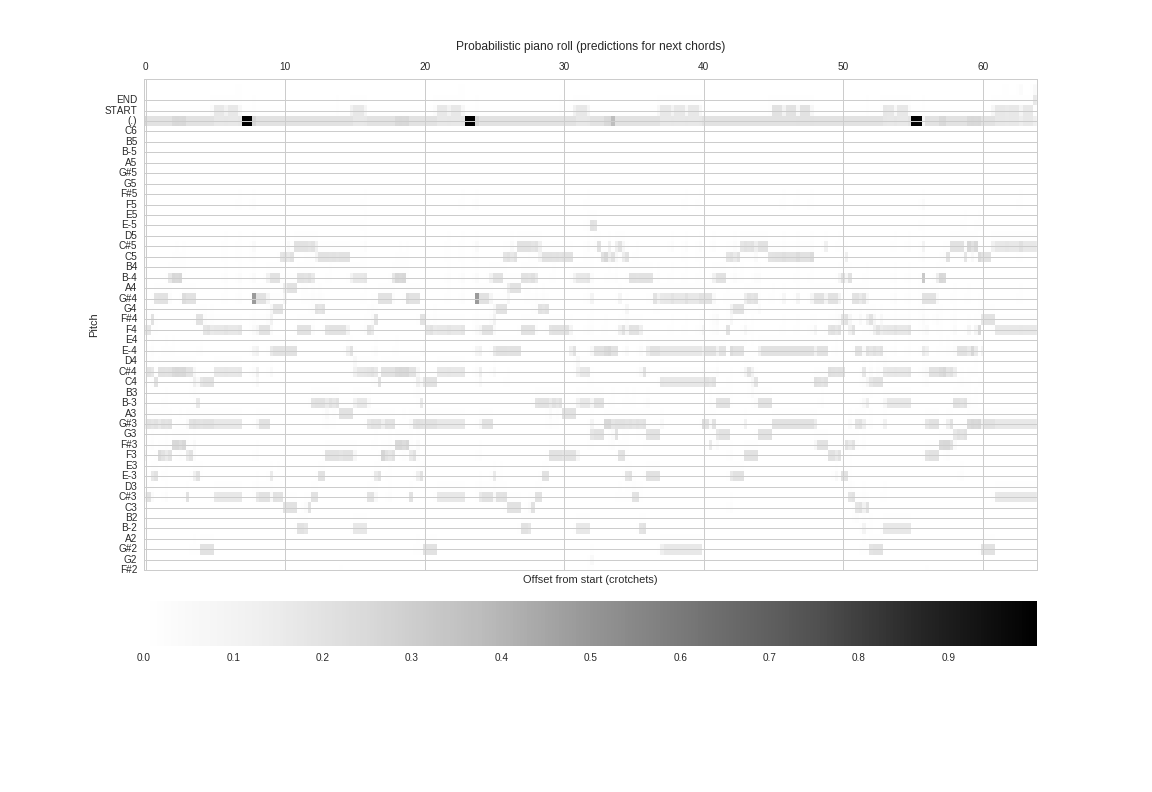
\includegraphics[trim={0 0 0 1.4cm},clip,width=0.995\linewidth]{Figures/model-analysis-probabilistic-piano-roll.png}
    \caption{Figures/model-analysis-probabilistic-piano-Roll}
    \label{fig:model-analysis-probabilistic-piano-roll}
\end{figure}

\subsection{Interesting neurons}

\begin{figure}[htpb]
    \centering
    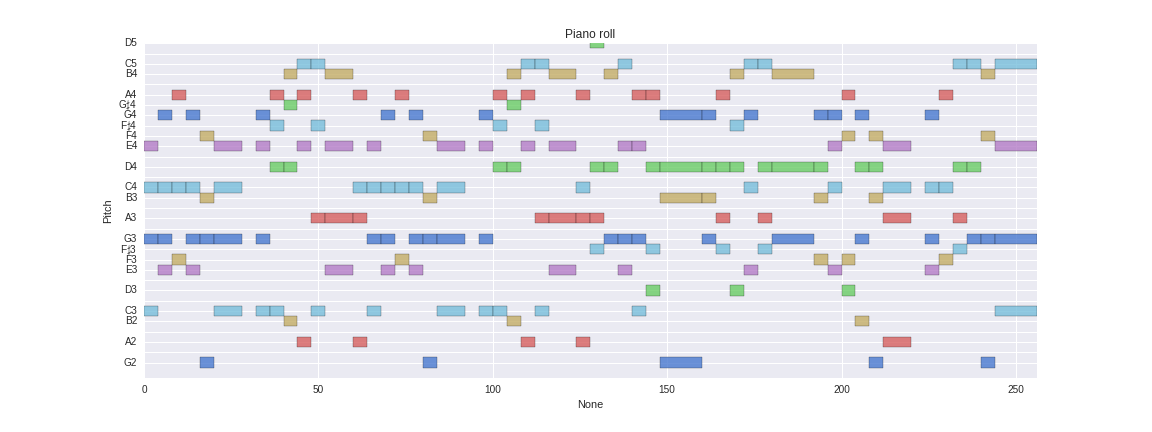
\includegraphics[width=1.0\linewidth]{Figures/model-analysis-cells-softmax-piano-roll.png}
    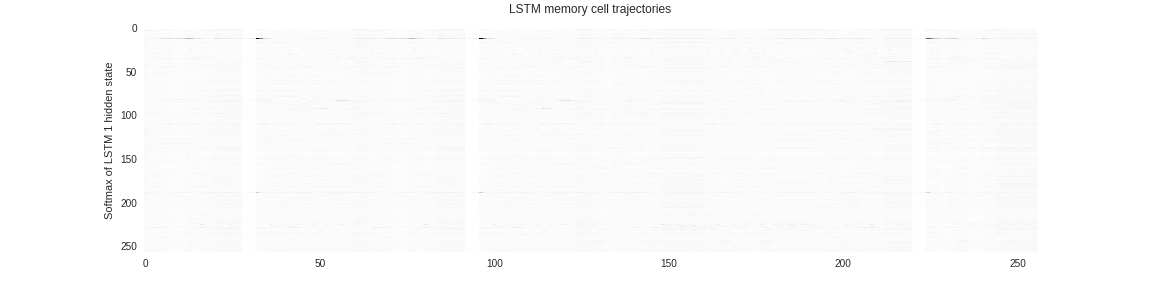
\includegraphics[width=1.0\linewidth]{Figures/model-analysis-cells-softmax-1.png}
    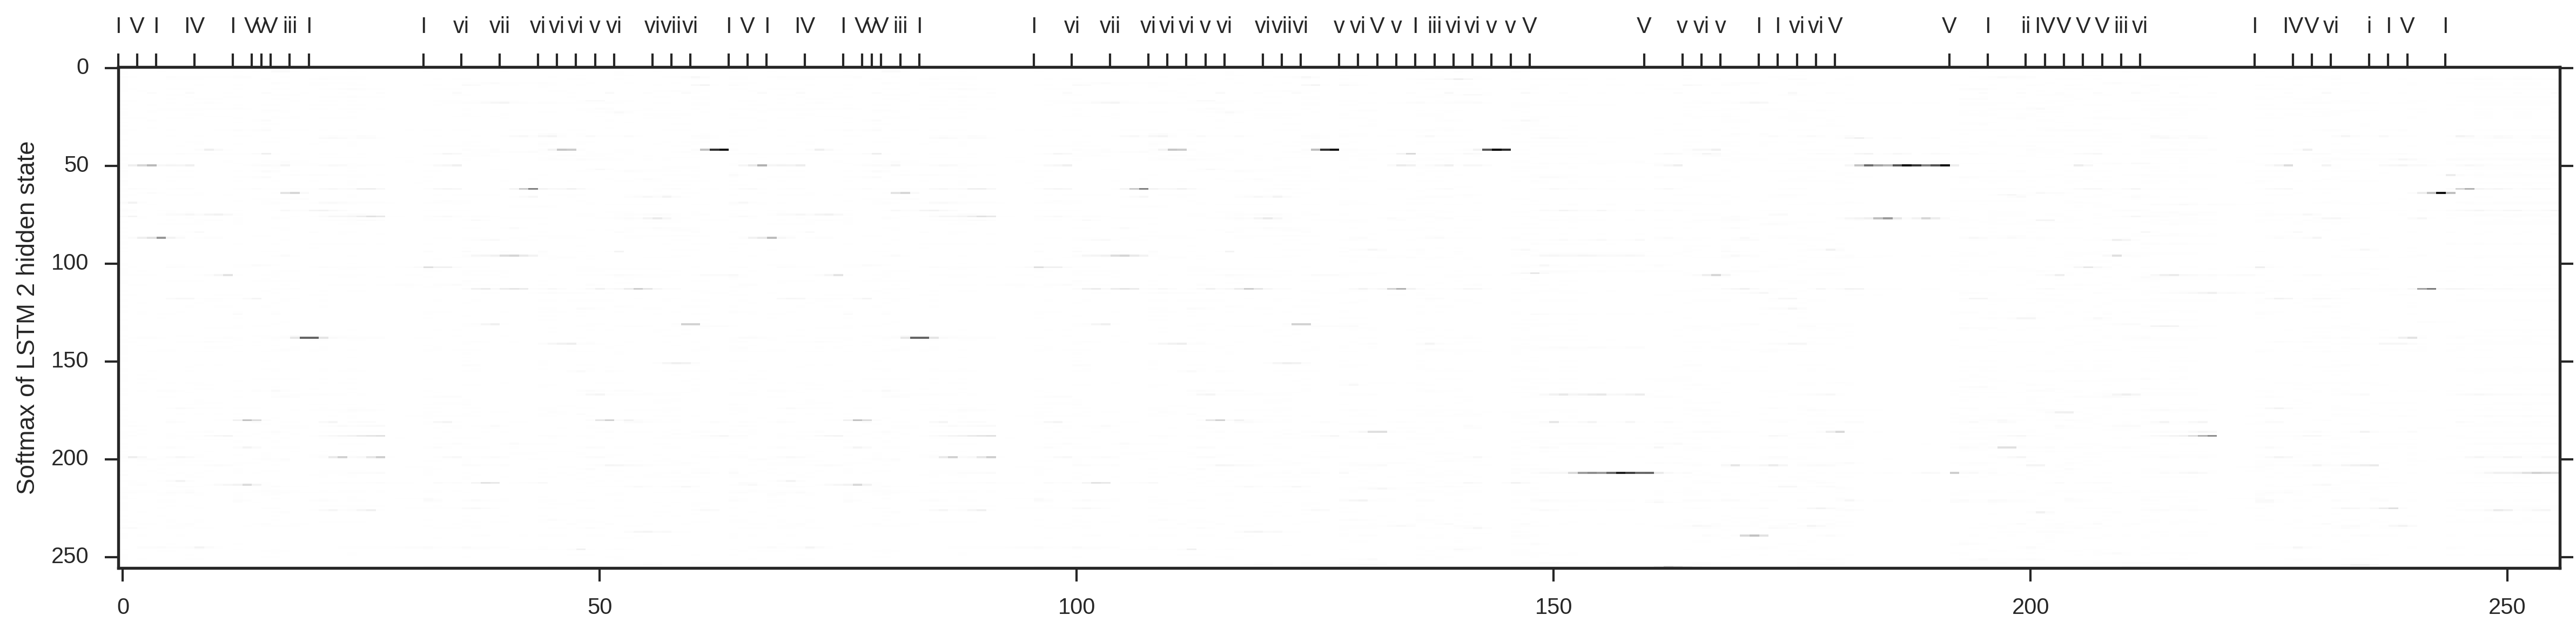
\includegraphics[width=1.0\linewidth]{Figures/model-analysis-cells-softmax-2.png}
    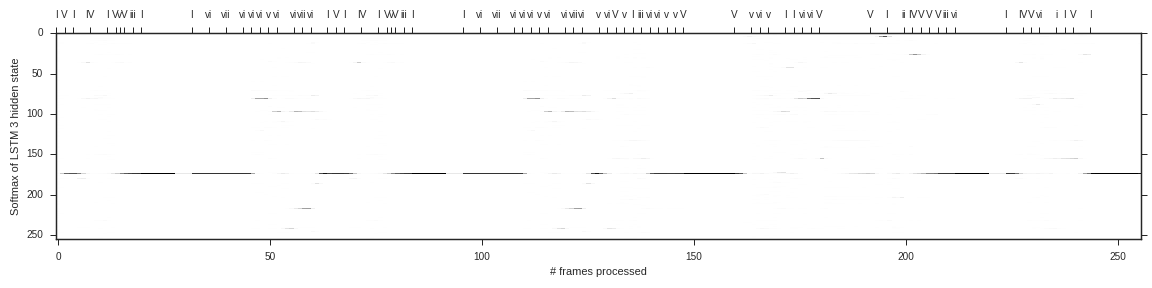
\includegraphics[width=1.0\linewidth]{Figures/model-analysis-cells-softmax-3.png}
    \caption{model-analysis-cells-Softmax}
    \label{fig:model-analysis-cells-softmax}
\end{figure}

\begin{figure}[htpb]
    \centering
    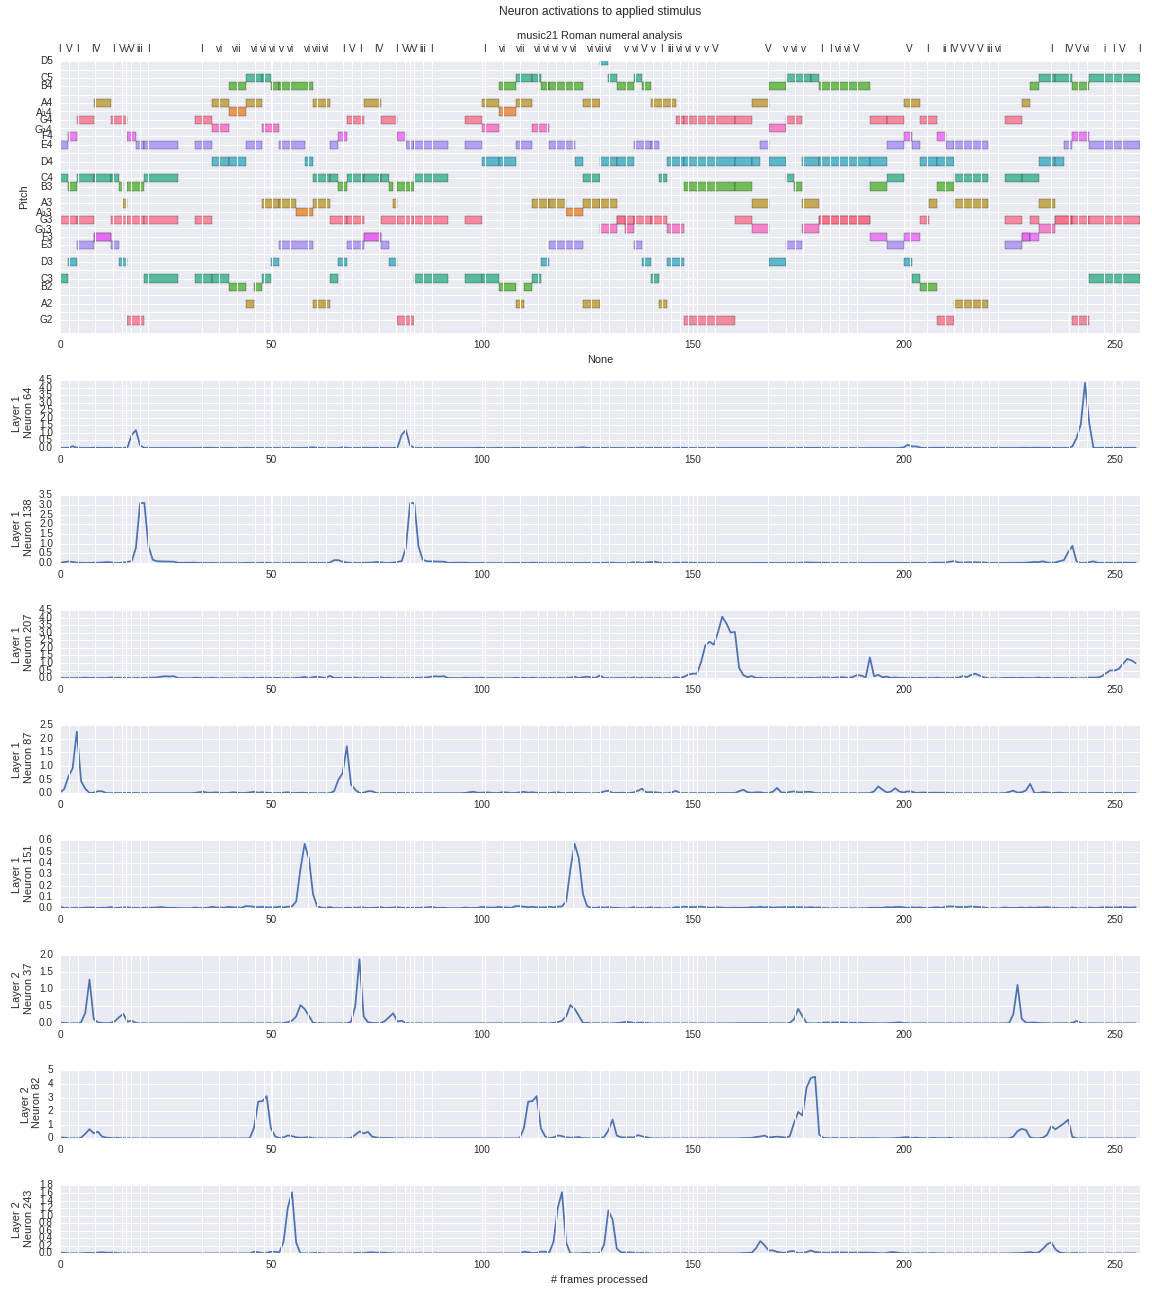
\includegraphics[width=1.0\linewidth]{Figures/model-analysis-cells-individual.png}
    \caption{Figures/model-analysis-cells-Individual}
    \label{fig:Figures/model-analysis-cells-individual}
\end{figure}


\printbibliography

\end{document}
